\documentclass
[12pt,
a4paper,
]{report}

\usepackage{ucs}
\usepackage[utf8x]{inputenc}
\usepackage[OT1]{fontenc}
\usepackage[frenchb]{babel}
\usepackage{lmodern}

\usepackage{makeidx}
\makeindex

\usepackage[rflt]{floatflt}
\usepackage{pdfpages}
\usepackage{url}
\usepackage{hyperref}
\hypersetup
{
	% bookmarks=true,
	unicode=true,
    pdfauthor={Habbachi Riadh},
    pdfsubject={Rapport de project de fin d'etudes},
    pdftitle={Mémoire de Projet de Fin d’Etudes-Développement d'une application Android pour médecins.},
    pdfkeywords={ENIG, Tunav, Stage, Stage ingenieur, project de fin d'etudes, LaTeX, PDF, hyperlinks}
}

\usepackage{cite}
\bibliographystyle{unsrt}

\usepackage{color}
\usepackage{xcolor}
\usepackage{listings}
\lstloadlanguages{
	XML,
	Java
}
\lstset{
	basicstyle=\footnotesize\ttfamily,
	breaklines=true
}
\usepackage{caption}
\DeclareCaptionFont{white}{\color{white}}
\DeclareCaptionFormat{listing}{\colorbox{gray}{\parbox{\textwidth}{#1#2#3}}}
\captionsetup[lstlisting]{format=listing,labelfont=white,textfont=white}

\usepackage[stable]{footmisc}

\usepackage{array}
% \usepackage{tablefootnote}

\usepackage{graphicx}
\usepackage{float}
\usepackage{wrapfig}
\usepackage{subfig}

\newcommand{\en}[1]{\textit{#1}}
\newcommand{\android}{Android\texttrademark}
\newcommand{\dev}[1]{\textit{#1}}
\newcommand{\pct}{PowerChart Touch\texttrademark}
\newcommand{\tm}[1]{\textbf{#1}\texttrademark}

\graphicspath{{../res/}}

\usepackage[nomain, toc,acronym]{glossaries}
%!TEX root = report.tex

%from documentation
%\newacronym[⟨key-val list⟩]{⟨label ⟩}{⟨abbrv ⟩}{⟨long⟩}
%above is short version of this
% \newglossaryentry{⟨label ⟩}{type=\acronymtype,
% name={⟨abbrv ⟩},
% description={⟨long⟩},
% text={⟨abbrv ⟩},
% first={⟨long⟩ (⟨abbrv ⟩)},
% plural={⟨abbrv ⟩\glspluralsuffix},
% firstplural={⟨long⟩\glspluralsuffix\space (⟨abbrv ⟩\glspluralsuffix)},
% ⟨key-val list⟩}

% A
\newacronym{api}{API}{Application Programing Interface}
% E
\newacronym{e-otd}{E-OTD}{Enhanced Observed Time Difference}
% G
\newacronym{gps}{GPS}{Global Positioning System}
\newacronym{gpx}{GPX}{GPS eXchange Format}
\newacronym{gsm}{GSM}{Global System for Mobile Communications}
% K
\newacronym{kml}{KML}{Keyhole Markup Language}
% L
\newacronym{lbs}{LBS}{Location Based Services}
% M
\newacronym{miaa}{MIAA}{Medical Information, Anytime, Anywhere}
\newacronym{mvc}{MVC}{model–view–controller}
\newacronym{mvp}{MVP}{model–view–presenter}
% S
\newacronym{sdk}{SDK}{Software Development Kit}
% T
\newacronym{tdoa}{TDoA}{Time Difference of Arrival}
\newacronym{ttm}{TTM}{Time-to-Market}
% U
\newacronym{uml}{UML}{Unified Modeling Langauge}
\newacronym{ui}{UI}{User Interface}
\newacronym{ux}{UX}{User Experience}
\makeglossaries

\author{Habbachi Riadh}
\title{Rapport de Projet de Fin d’Étude}

\usepackage{fancyhdr}
\setlength{\headheight}{16pt}
\fancyhf{}
\pagestyle{fancyplain}
\fancyhead[L]{\textbf{ENIG}}
\fancyhead[R]{\textbf{TUNAV}}
\fancyfoot[L]{\textsc{Habbachi Riadh}}
\fancyfoot[R]{\thepage{} / \pageref{LastPage}}

\begin{document}


\includepdf[pages=-]{page_de_garde_pfe_2013.pdf}

\tableofcontents
\listoftables
\listoffigures

\glsaddall
\printglossary[type=\acronymtype,title={Liste d'Abréviations},toctitle={Liste d'Abréviations}]

%!TEX root = report.tex

\chapter{Introduction Général}

Ces temps ci, le mobile s’est imposé et devient la norme pour les
consommateurs. Les statistiques ne le cachent pas, c’était prévisible,
mais tous les analystes le soulignent: "Le marché des PC s’effondre face
aux smartphones et aux tablettes"\cite{lefigaro}. Et un des secteurs qui
pourrait bénéficier de l'avalanche des systèmes mobile est le secteur
médical.

Les applications mobiles offrent un potentiel énorme pour supporter et
activer des nouvelles opportunités pour les services médicaux.
Localisation, instantanéité, efficacité, personnalisation et une très
grande accommodation vont offrir plusieurs moyens nouveaux pour
améliorer l’expérience des services médicaux, du côté du patient
sûrement, mais tend aussi à rendre l’établissement plus convivial pour
les médecins et en général le staff médical.

Investir dans une application mobile représente pour les hôpitaux, et
les institutions qui les implémentent, un autre moyen pour étendre les
outils numériques déjà en place, en offrant des fonctionnalités qui sont
auparavant cloué aux ordinateurs des administrations. Ceci  facilitera
le processus de traitement des malades.

Cependant, l’usage des smartphone dans les établissements est sujet aux
questions notamment sur le plan technique. Les technique d’accès et de
sécurisation des données des patients et divers technologies utilisés et
surtout le manque de standardisation pose un sérieux challenge pour les
entreprises voulant offrir des solutions pour les établissements
médicaux.

Dans ce même thème se présente ce projet de fin l’étude sur la
conception et développement d’une application mobile sur plate-forme
Androïd destiné aux médecins dans le but de faciliter l’accès aux
dossiers médicaux des patients en intégrants les techniques de
localisation. Ce rapport est subdivisé en trois parties: La première
partie expose le cadre général du projet en présentant l’entreprise hôte
ainsi que les objectifs de l’application. La deuxième partie évoque les
solutions similaires déjà présentes dans le marché ainsi que une
présentation de la plate-forme sur la quelle l’application est à
développer. La troisième et dernière partie décortique le travail
effectué pour accomplir les objectifs.

%!TEX root = report.tex

\chapter{Cadre Général du Projet}

\section{Introduction du Chapitre}

Ce chapitre est subdivisé en deux parties: la première partie est
consacrée à la présentation de l’organisme d’accueil \textbf{TUNAV}. La
deuxième partie est destinée à la présentation du projet en soit.

\section{Présentation de l'organisme d'accueil}  

\begin{figure}
\center

\includegraphics[scale=1]{tunav-logo}
\caption{Logo \textsc{Tunav}.}
\end{figure}

TUNAV se situe à la Cité Technologique des Communications, Parc
Technologique El Gazala à l’ARIANA, et a été fondée par son Président
Directeur Général Mohamed Anis Kallel.

En guise de présentation, rien de mieux que de l’avoir directement du patron lui-même\cite{index_tunisie}:

"\textsc{Tunav} est une société technologique, créée au mois d’août
2004, implantée à la technopole El Gazala et spécialisée dans la
technologie GPS et ses diverses applications dans les domaines de
navigation et de gestion de flotte."

"\textsc{Tunav} est connue en Tunisie par son système \og{}LaTrace\fg{}
de gestion de flotte par GPS, lequel a été commercialisée pour la
première fois en Octobre 2005. Il s'agit d'un système articulé autour
d'une application très évoluée de gestion de flotte, d'une gamme
d'appareils GPS/GPRS et d'une base de données géographique richement
renseignée."

\textsc{Tunav} possède un savoir faire reconnu dans le domaine de la
localisation qui peut être exploité dans le domaine médical.

\section{Présentation du projet}

Ce projet s'inscrit dans un effort pour faciliter le travail des médecins en
leurs rapprochant de leur patient à travers des technologies de localisation.
chaque médecin authentifier a accès à la liste de ses patients ordonner dans
l'ordre de leur cas (urgent ou non), leur proximité géographique dans
l’établissement, et leur date d’admission dans l'hôpital. L'application doit
être conçu de manier a accommodé au différentes configuration des clients
potentiels avec des modifications minimales.

Cette application vise \underline{principalement} les médecins. Et
malgré que, suite à des choix conceptuels, rien n’empêche qu’avec des
modifications minimes une audience plus large dans le corps médical
pourra être ciblée, ce n’est pas -pour le moment- le but de
l’application. Les médecins, malgré leur formation prolongé dans le
domaine médical, représente une cible sans une vraie profondeur
technique, ce que requit de l’application d’être le plus simple
possible.

%!TEX root = report.tex

\chapter{État de l'art}
\section{Introduction}

Dans ce chapitre on présente une étude du marché en énumérant les
applications dont les fonctionnalités sont équivalentes à la notre tout
en soulignant les différences qui subsistent. Ensuite on présente la
plate-forme ciblé et en passe en revu l’architecture d’une application
\android{}.

\section{Étude de marché}

Plusieurs sociétés offrent des solutions en relation avec celle proposé
par ce présent rapport. Malheureusement, la plupart d’entre elles sont
des solutions commerciales et, faute de documentation disponible, on n’a
pas pu les étudier d’un point de vu techno-technique et on s’est
contenté de relayer leurs caractéristiques tel que présenté dans les
sources cités.

\paragraph{NB:} % (fold) 
\label{par:nb}

Les solutions présentées ici sont le fruit des sociétés bien établis avec des ressources considérables et des salariés professionnels. Les comparer avec le travail incubé dans ce rapport serai abusif, l’indulgence est de mise.

\subsection{MIAA - Palomar Pomerado Health}

\begin{figure}
\centering
\subfloat{
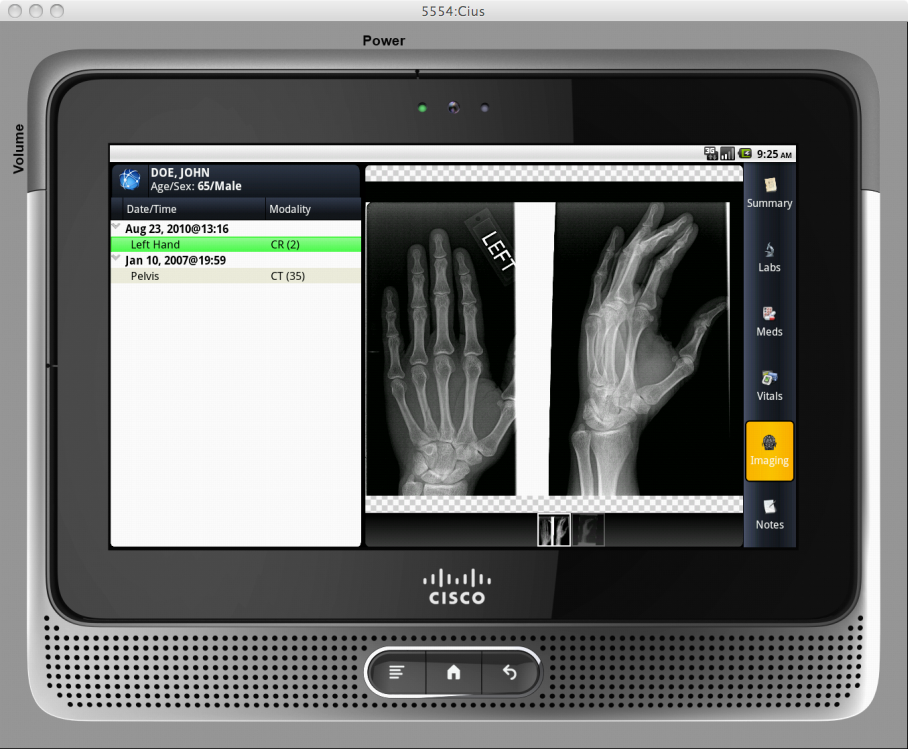
\includegraphics[width=0.5\textwidth]{pph1}
}\\
\subfloat{
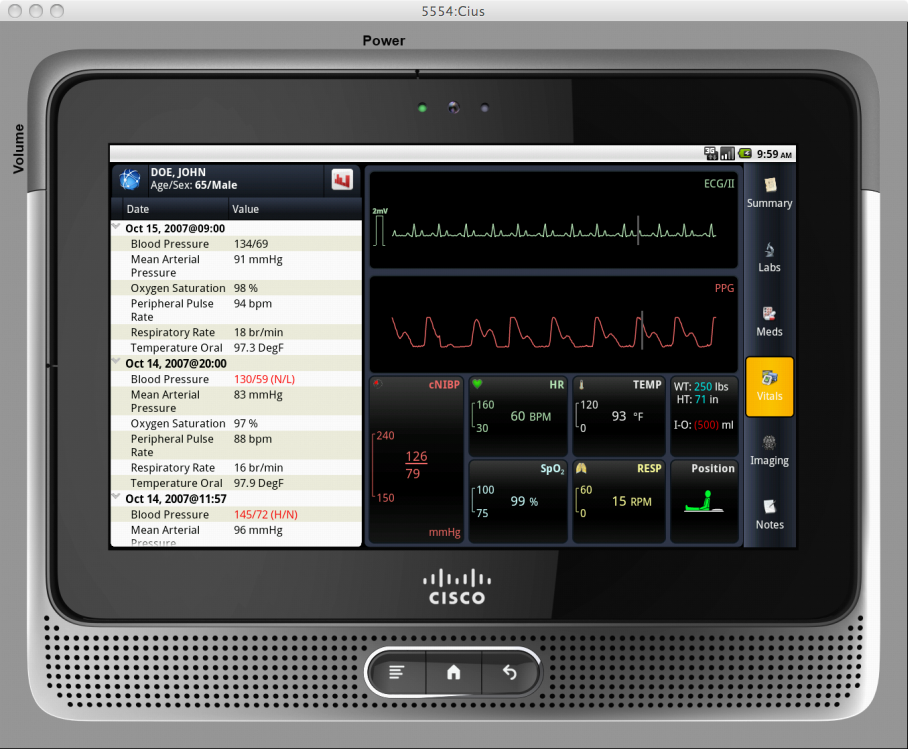
\includegraphics[width=0.5\textwidth]{pph2}
}\\
\subfloat{
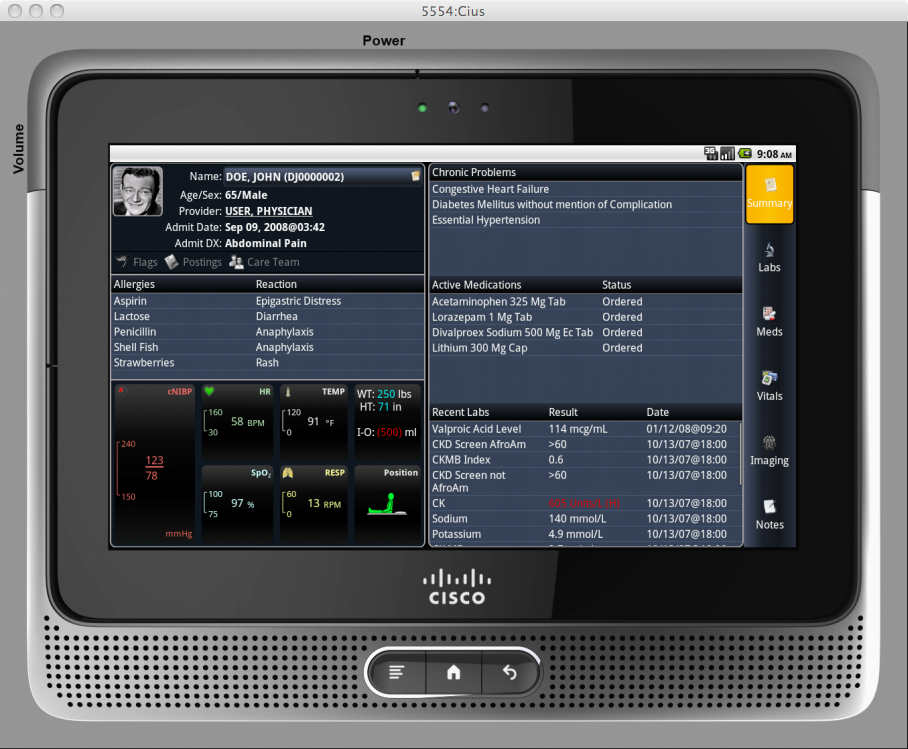
\includegraphics[width=0.5\textwidth]{pph3}
}
\caption{\gls{miaa} sur un émulateur Cisco Cius}
\label{fig:miaa}
\end{figure}

\gls{miaa} (figure \ref{fig:miaa}) est une application mobile issu d'un
projet R\&D chez \en{Palomar Pomerado Health}, l'institution public la
plus large dans l'état de Californie (USA). Elle permet aux médecins
d'accéder rapidement au dossier médical complet du patient depuis une
variété de source différentes qui s'affranchie des frontières des
organisations\cite{pph:eweek}. Elle vise les terminaux équipés avec le
système d'exploitation \android{} comme les smartphones et les
tablettes. \en{Palomar Pomerado Health} a choisi de déployer cette
application dans le \en{Palomar Medical Center} à \en{Escondido} (319
lits) et le \en{Pomerado Hospital} à \en{Poway} (107 lits) sur des
tablettes Cisco Cius\cite{pph:tabtimes}, ce choix s'est basé sur le
support qu'offre Cisco pour ces équipements.

Les avantages de \gls{miaa} sont:~\cite{pph:yahoo}

\begin{itemize}

\item Application mobile facile à utilisé conçu spécifiquement aux
médecins, tournant sur la plate-forme \android{}.

\item Un service \en{Cloud} qui fournit un accès permanent à
l'historique médicale des patients à partir de divers sources de
données qui s'affranchie des frontières des organisations.

\item Interopérabilité avec les pionniers des systèmes électroniques
de l'historique médical tel que Cerner - \tm{Millennnium},
\tm{NextGen}, et \en{Veterans Administration} - \tm{VistA}.

\item Intégration en temps-réel des technologies de surveillance
des signes vitaux sans fils comme l'ECG, SPO$_{2}$, rythme cardiaque,
température, respiration, et pression du sang à partir des équipements
sans-fils.

\item Affichage des informations génétiques personnelles.

\item Application dynamique qui s’ajuste automatiquement à l’hôpital, clinique, et à la maison.

\item Simple, facile à utiliser, avec une tactile de nouvelle génération.

\item Intégration d’une messagerie inter-médecins sécurisée tout en maintenant le contexte du patient.

\item Des plan futurs pour intégré NHIN \en{Connect} et les services
\en{Direct}.

\end{itemize}

\subsection{\pct{} - Cerner}

\begin{figure}[H]
\centering

\includegraphics[width=0.3\textwidth]{logo_cerner}
\end{figure}

\pct{} est une solution mobile conçu par le laboratoire Cerner qui
fait parti de l'ensemble de solutions \tm{Millennium+} et qui permet de
facilité le travail des médecins. Elle offre une expérience native
sur iPad pour gérer les visites médicales et permet aux médecins
d'effectuer tout une visite typique qui inclue:~\cite{pct:flyer}

\begin{itemize}

\item Consultation des emplois du temps et les chartes des patients.

\item Satisfaire les demandes récurrentes comme les commandes simples
et les recharges des médicaments.

\item Consultation des diagnostiques et résultats cliniques.

\item Documenter les allergies, les problèmes de santé et l'historique
du patient.

\item Crée et signé les notes de progressions.

\end{itemize}

Dès la fin du flux de travail du médecin ambulant. Cerner étend ces
mêmes fonctions et les adaptes aux établissements hospitaliers, les
urgences et les divers spécialistes.
Les avantages clés du \pct{} sont:~\cite{pct:flyer}

\begin{itemize}

\item Des réponses instantanées avec un flux de travail aisé.

\item Pas besoin de configurer l'application.

\item Adapter pour les visites médicales, aux patients et aux conditions
de la consultation.

\item Transmission sécurisée des données.

\item Des capacités de reconnaissance vocale.

\end{itemize}

\section{Le système d'exploitation \android{}}

\begin{figure}[H]
\begin{center}

\includegraphics[width=0.2\textwidth]{Android_robot.pdf}\\

\includegraphics[width=0.2\textwidth]{Android.pdf}
\end{center}
\caption{Logo et sigle d'\android{}}
\end{figure}

\android{} est un système d'exploitation basé sur Linux conçu pour les
équipements mobile avec d'un écran tactile comme les \en{smartphones} et
les tablettes. Développé à l'origine par \en{\android{}, Inc.} que
\en{Google} a supporté financièrement et plus-tard acquis en 2005.
\android{} a été dévoilé en 2007 parallèlement à la fondation de
l'\en{Open Handset Alliance}: un consortium composé de sociétés dévoué a
l'avancement des standards ouverts pour les équipements mobiles. Le
premier téléphone  \android{} est sorti en Octobre 2008.

La dernière version stable d'\android{} en date (Mai 2013) est 4.2.2
\en{Jelly Bean} sortie le 11 Février 2013.

\android{} est basé sur le Kernel Linux et utilise pleinement ses capacités de supports matériels exhaustifs. Mais la comparaison avec les distributions Linux, embarqué ou même destiné aux bureaux, s'arrête à ce niveau.~\cite{lft:growth_android}

\begin{figure}
\centering
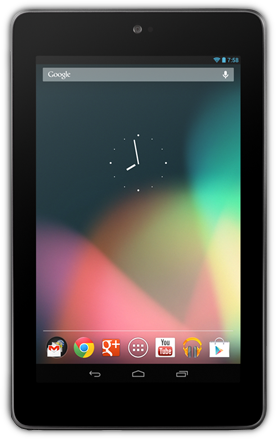
\includegraphics[width=0.4\textwidth]{nexus7}
\caption{\en{Google} Nexus 7, un terminal \android}
\end{figure}

\subsection{Parts du marché}

L’adoption du système d'exploitation \android{} suit une courbe
exponentielle depuis quelque temps et la tendance n'est pas prête de
s’inverser, selon le dernier rapport du cabinet d'analyse \en{Strategy
Analytics}, \android{} a réussi à capturer environ 68.4\% du marché
global \cite{venturebeat.com}.

\begin{table}[H]
\centering
\begin{tabular}{|m{0.2\textwidth}|m{0.13\textwidth}|m{0.13\textwidth}|m{0.13\textwidth}|m{0.13\textwidth}|m{0.13\textwidth}|}
\hline
\textsf{Système d'exploitation} &
\textsf{Volume de production 3Q2012\footnotemark[1]\footnotemark[3]} &
\textsf{Parts du Marché 3Q2012\footnotemark[1]} &
\textsf{Volume de production 3Q2011\footnotemark[2]\footnotemark[3]} &
\textsf{Parts du Marché 3Q2011\footnotemark[2]} & \textsf{Différence} \\ 
\hline
\android{} & 136.0 & 75.0\% & 71.0 & 57.5\% & 91.5\% \\
\hline
iOS & 26.9 & 14.9\% & 17.1 & 13.8\% & 57.3\% \\
\hline
BlackBerry & 7.7 & 4.3\% & 11.8 & 9.5\% & -34.7\% \\
\hline
Symbian & 4.1 & 2.3\% & 18.1 & 14.6\%  & -77.3\% \\
\hline
Windows Phone 7/ Windows Mobile & 3.6 & 2.0\% & 1.5 & 1.2\% & 140.0\% \\
\hline
Linux & 2.8 & 1.5\% & 4.1 & 3.3\% & -31.7\% \\
\hline
Autres & 0.0 & 0.0\% & 0.1 & 0.1\% & -100.0\% \\
\hline
\hline
Totales & 181.1 & 100.0\% & 123.7 & 100.0\% & 46.4\% \\ \hline
\end{tabular}

\caption{Les six major systèmes d'exploitation mobile en termes de Volume
et de parts de marché en 3\ieme trimestre 2012~\cite{idc}}

\label{tab:marketshareall}
\end{table}

\footnotetext[1]{3\ieme trimestre 2012}
\footnotetext[2]{3\ieme trimestre 2011}
\footnotetext[3]{En million d'unité}

\begin{table}[H]
\centering
\begin{tabular}{|m{0.3\textwidth}|m{0.1\textwidth}|m{0.1\textwidth}|m{0.1\textwidth}|m{0.1\textwidth}|m{0.1\textwidth}|}
\hline
& \textsf{2008} & \textsf{2009} & \textsf{2010} & \textsf{2011} &
\textsf{2012}\footnotemark[4]\\
\hline
\textsf{Unités \android{} produites} & 0.7 & 7.0 & 71.1 & 243.4 & 333.6\\
\hline
\textsf{Parts de marché \android{}} & 0.5\% & 4.0\% & 23.3\% & 49.2\%
& 68.2\%\\
\hline
\end{tabular}
\caption{Production et parts de marché entre 2008 et 2012~\cite{idc}}
\label{tab:marketshare}
\end{table}

\footnotetext[4]{Estimation}

\subsection{Versions \android{} en circulation}

Le tableau \ref{tab:androidversion} représente les différentes versions
d'\android{} et leurs taux d'utilisation respectifs. On remarque que
la plupart des terminaux mobiles \android{} sont sous la version 2.3
\en{Gingerbread} sortie le 6 Décembre 2010, Ceci est du aux fait que
plusieurs téléphones bas de gamme sont équipés de cette version et sont encore en production.

\begin{table}[H]
\centering
\begin{tabular}{|c|l|c|c|}
\hline
\textsf{Version} & \textsf{Codename} & \textsf{API} &
\textsf{Distribution}\\
\hline
1.6 & Donut & 4 & 0.2\%\\
\hline
2.1 & Eclair & 7 & 2.2\%\\
\hline
2.2 & Froyo & 8 & 8.1\%\\
\hline
2.3 - 2.3.2 & Gingerbread & 9 & 0.2\% \\
\cline{1-1}\cline{3-4}
2.3.3 - 2.3.7 & & 10 & 45.4\%\\
\hline
3.1 & Honeycomb & 12 & 0.3\%\\
\cline{1-1}\cline{3-4}
3.2 & & 13 & 1.0\%\\
\hline
4.0.3 - 4.0.4 & Ice Cream Sandwich & 15 & 29.0\%\\
\hline
4.1 & Jelly Bean & 16 & 12.2\%\\
\cline{1-1}\cline{3-4}
4.2 & & 17 & 1.4\%\\
\hline
\end{tabular}
\caption{Distribution des versions \android{} en circulation qui ont
accédé au \en{Google Play}\protect\footnotemark[5]}
\label{tab:androidversion}
\end{table}

\footnotetext[5]{Données récoltées pendant une période de tests de 14
jours arrêtée le 4 Février 2013.}
%%%ENDsubsection

\subsection[Les raisons du succès d'\android{}]{Les raisons du succès d'\android{}\cite{lft:growth_android}}

Les raisons pour le succès \android{} peuvent être
dénombrées comme suit:

\begin{description}

\item [Un \en{Framework} d'Application Riche.] \android{} fourni un
excellent \gls{sdk} avec des \gls{api} stable à long-terme, ce qui
assure aux partenaires tiers un écosystème standardisé. Alors que le
système en lui même est en constante évolution, la stabilité des
\gls{api} pour la plupart est préservée, ce qui permet d'investir dans
le long-terme. Concevoir et construire des applications pour les
distribuer sur différentes plate-formes permet des réductions drastiques en
termes des coûts et effort pour les entreprises.

\item [Un \gls{ttm} Agressif.] Concevoir des appareils avec \android{}
peut réduire le \gls{ttm} d'une manière significative. Il suffit de se
procurer les sources, les adapter pour le matériel en question et vendre. Et dans le cas ou les schémas et usages de référence sont
appliqués, la sorti d'un nouveau produit est possible au cours de quelque
mois. Seulement voilà, ce n'est pas aussi facile et une certaine expertise
et connaissances dans ce domaine sont requises. Et même si sortir un
système basé sur \android{} peut être plus rapide comparé à d'autres
solutions, le suivi des évolutions du système ainsi que maintenir le
code à long terme est une autre histoire.

\item [Concentrer sur \og Ce qui compte réellement \fg.] En fournissant
un \en{Framework} pratique, \android{} permet aux développeurs de se
concentrer sur les aspects à valeur commerciale. L'assemblage d'un
appareil est une activité qui consomme énormément de temps et de
ressources et n'a pas à réinventer un - encore - autre système d'exploitation permettant d'éviter un autre gaspillage de temps.

\item [Open Source.] Bien qu'il ne soit pas développé d'une manière
communautaire, \android{} reste 100\% modifiable et diffuse un sentiment
de sécurité parmi les entreprises contre les menaces légales.

\end{description}

\subsection[La pile logicielle d'\android{}]{La pile logicielle d'\android{}\cite{pa4ad:chptr1}}

D'une manière simple. La pile logicielle d'\android{} est un Kernel Linux et une collection de bibliothèques C/C++ exposé à travers un framework d'application qui fournit des services pour l'environnement d'exécution et les applications. On peut énumérer les éléments composant la pile logicielle comme suit:

\begin{description}

\item [Kernel Linux:]
Services de base qui inclue les pilotes matériels, gestion des processus et de la mémoire, sécurité, réseaux et gestion d'autonomie. Fourni aussi une couche d'abstraction entre le matériel et le reste de la pile.

\item [Bibliothèque:]
Se situ au dessus du Kernel, \android{} inclue divers bibliothèques C/C++ de base comme \dev{libc} et \dev{SSL} ainsi que:

\begin{itemize}

\item Une bibliothèque multimédia pour la lecture des fichiers audio et vidéo.

\item Un \en{Surface manager} pour la gestion de l'affichage.

\item Des bibliothèques graphiques qui incluent le \dev{SGL} et \dev{OpenGL} pour les graphiques 2D et 3D.

\item Un support natif de base de données à travers la base de données \dev{SQLite}.

\item \dev{SSL} et \dev{WebKit} pour le navigateur web intégrer et la sécurité internet.

\end{itemize}

\item [Environnement d'Execution (runtime) \android{}:]

L'environnement d’exécution et le facteur qui sépare un terminal \android{}
d'une implémentation Linux mobile. En cohérence avec les bibliothèques de base
et la machine virtuelle \dev{Dalvik}, l'environnement d’exécution \android{} est
le moteur qui fait fonctionner les applications et, avec les bibliothèques,
forme les bases du framework application.

\begin{description}

\item [Bibliothèque de Base:]

Même si la plus part des applications \android{} sont écrits avec du langage
\dev{Java}, \dev{Dalvik} n'est pas une machine virtuelle java. Les bibliothèques
\android{} de base fournit la plus part des fonctionnalités qu'on retrouve
dans les bibliothèques de base \dev{Java}, en plus de quelque bibliothèques
spécifiques à \android{}.

\item [La Machine Virtuelle dev{Dalvik}:]

\dev{Dalvik} est une machine virtuelle qui a était optimisé pour
s'assurer que chaque terminal peut faire fonctionner plusieurs instance
d'une manière efficace. Il s’appuie sur le Kernel Linux pour le
threading et la gestion bas niveaux de la mémoire.

\end{description}

\item [Le \en{Framework} Application:]

Le \en{Framework} application fournit les classes utilisés pour crée les application \android{}. Il fournit une abstraction générique pour l’accès matériel et gère l'\gls{ui} et les ressources de l'application.

\item [Couche Application:]

Toutes les applications, quelle soit native ou produite par un tiers, est
construites sur la couche applications via les même \gls{api}. La couche
application opère à l'intérieur de l'environnement d’exécution \android{},
utilisant les classes et les services mise à disposition par le \en{framework}
application.

\end{description}

\subsection[Architecture des applications \android{}]{Architecture des applications \android{}\cite{pa4ad:chptr1}}

L'architecture d'\android{} encourage la réutilisation des composants,
ce qui nous permet de publier et de partager des \en{Activities},
services, et données avec d'autres applications. Avec une gestion
d'accès gérée par les restrictions de sécurité que nous définissons.

Le même mécanisme qui nous permet de produire un gestionnaire de contact alternatif ou un compositeur de numéros nous permet aussi d'exposer les composants de notre application pour permettre à d'autres développeurs de les réutiliser en créant des nouveaux \gls{ui} ou d’étendre des fonctionnalités.

Les services application suivants représente les bases architecturales de toute application \android{}, fournissant le \en{Framework} qu'on va utiliser pour notre application.

\begin{description}

\item [L'\dev{Activity Manager} et le \dev{Fragment Manager}:]
Contrôle le cycle de vie de nos \en{Activities} et nos \en{Fragments} respectivement, y inclue la gestion de la pile des \en{Activities}.

\item[\dev{Views}]
Utilisé pour construire l'\gls{ui} de notre \dev{Activities} et \dev{Fragments}.

\item[\dev{Notification Manager}:]
Fournit un mécanisme consistant et non-intrusif de signalisation pour l'utilisateur.

\item[\dev{Content Providers}:]
Permet à notre application le partage des données.

\item[\dev{Resource Manager}:]
Offre un moyen d'externaliser les ressources (comme par exemple les chaînes de caractères et les images.)

\item[\dev{Intents}:]
Présente un mécanisme pour transférer les données entre les applications et leurs composants.

\end{description}

Une des fonctionalités les plus intéressantes pour l'aboutissement de notre projet offerte par \android{} sont ses capacités de localisation, étudiées dans la partie suivante.

\subsection{Location Based Services}

\subsubsection{Concept}

Pour positionner un terminal, on spécifie ses coordonnées géographiques
en utilisant le géo-codage.

\paragraph[Géo-codage]{Géo-codage\cite{wiki:geocoding}}

Le géo-codage est le processus de retrouver les coordonnées
géographiques associées (exprimées souvent en terme de \textit{latitude}
et \textit{longitude}) d'après d'autre données géographiques comme
l'adresse de la rue, code postal. Ces coordonnées géographiques peuvent
être insérées dans un système d'informations géographiques ou intégré dans
des médias comme les photos numériques par le biais de géo-marquage.
Cette opération est communément appelé le \en{Forward Geocoding}.

Le \en{Reverse Geocoding} est la procédure inverse: retrouvé les lieux textuel comme l'adresse de la rue d'après les coordonnés géographiques. Car même si l'usage des paramètres comme la longitude et la l'attitude fourni un moyen pratique pour localisé l'individu d'une maniéré relativement précise. Les utilisateurs penche à pensés en terme de rues et adresses.

A fin de déterminer la position du terminal, plusieurs technologie de localisation sont à notre disposition.

\paragraph[Localisation par GSM]{Localisation par GSM}

On peut retrouver la position du terminal mobile par le biais de sa
cellule \gls{gsm}. Cette technique fait intervenir divers moyens de
triangulation des signaux parvenant depuis les cellules qui desservent
un téléphone mobile. La position géographique du terminal est déterminée
par une multitude de méthodes comme la \gls{tdoa} ou l'\gls{e-otd}.

\paragraph[Localisation parGPS]{Localisation parGPS\cite{enig:gps}}

\gls{gps} est un système de navigation par satellites qui fourni la
localisation et le temps dans toute condition météorologique et partout
sur terre s'il existe un accès non bloquant à 4 ou plus satellites
\gls{gps}. Ce Système fourni des services essentiels dans le domaine
militaire, civil et commercial partout dans le monde. Il est maintenu
par les États Unis d'Amérique et accessible à quiconque possédant un
récepteur \gls{gps}.

\subsubsection[La localisation dans \android{}]{La localisation dans \android{}\cite{pa4ad:chptr13}}\label{sss:android_localisation}

L'accès aux \gls{lbs} se fait essentiellement via deux objets:
\begin{description}
\item [\dev{Location Manager}]\footnote{android.location.LocationManager} Permet d'exploiter les services basés sur la localisation.
\item [\dev{Location Providers}]\footnote{android.location.LocationProvider} Chaque \en{Providers} représente une technologie de localisation utilisé afin de déterminer la localisation actuel du terminale.

\end{description}
On utilise ces deux Classes pour les fins suivantes:
\begin{itemize}
\item Obtenir la position actuelle.
\item Suivre les mouvements.
\item Alerte de proximité dans le cas ou l'on approche ou s’éloigne d'une zone spécifique.
\item Retrouver les fournisseurs de localisation disponible.
\item Observer le status du récepteur \gls{gps}.
\end{itemize}

Généralement deux techniques de détection de localisation sont disponibles dans le terminal: détection par le réseau \en{Network Provider} et la détection par \gls{gps} (\en{GPS Provider}). Le choix de la technologie à utiliser est soit explicite ou automatique suivant des critères prédéfinis par le développeur de l'application. Avant de pouvoir exploiter un service de localisation, un niveau de précision doit figurer dans le manifeste de l'application via les \dev{uses-permission} \en{tags}.

\paragraph{Niveau de permission \textbf{COARSE} } % (fold)
\label{par:coarse}

\begin{lstlisting}[language=xml, caption=Permission pour la localisation par le réseau.]
<uses-permission android:name="android.permission.ACCESS_COARSE_LOCATION"/>
\end{lstlisting}
% paragraph par:coarse (end)

\paragraph{niveau de permission \textbf{FINE} } % (fold)
\label{par:fine}

\begin{lstlisting}[language=xml, caption=Permission pour la localisation par GPS.]
<uses-permission android:name="android.permission.ACCESS_FINE_LOCATION"/>
\end{lstlisting}

A noter qu'une application ayant la permission \dev{FINE} possède implicitement la permission \dev{COARSE}.

Avoir la localisation dans la plat-forme \android{} se fait par le biais de
\en{callback}, on indique au \dev{LocationManager} qu'on veut recevoir des mise
à jour de la localisation par la fonction \dev{requestLocationUpdates()} en lui
passant une implémentation de
\dev{LocationListener}\footnote{android.location.LocationListener}. Cette
interface contient plusieurs fonctions de \en{callback} que le
\dev{LocationManager} appelle quand la localisation de l'utilisateur change ou
l'état du service change\cite{guide:location_strategies}.


\section{Conclusion}

Dans ce chapitre, on s'est permis d'inspecter les solutions similaires à
la notre dans le but de s'éclaircir les idées sur les problèmes qu'on
pourrait rencontrer et pour mieux cerner les difficultés que nous allons
rencontré. Vient en suite la présentation de la plate-forme ciblée en
plus d'une application type, des connaissances critiques pour le chapitre
suivant qui porte sur le travail effectué.

%!TEX root = report.tex

\chapter{Travail Accompli}
\section{Introduction du chapitre}
Dans ce chapitre on procéde à la presentation des cas utilisateur de notre systéme ainsi que l'identification des acteurs impliqué dans ces cas. Puis on décortique l'implementation que nous proposant en citant eventuellement nos motifs et intentions.

\section{Vue Général}
\subsubsection{Identification des acteurs}
Notre systéme interagie essentiellement avec trois acteurs différents:
\begin{description}
\item[Le medecin] C'est l'acteur principale de notre systéme.

\item[Le service web] Source des données à achiminé vers le medecin
(Tache et )

\item[Systéme d'exploitation] Communique à notre systéme les information
receuille des divers composants qui nous interresse (localisation
GPS/Network, etat de la connectivité, etat de la battery).

\end{description}

\subsection{Cas d'utilisations}

\begin{figure}
\center
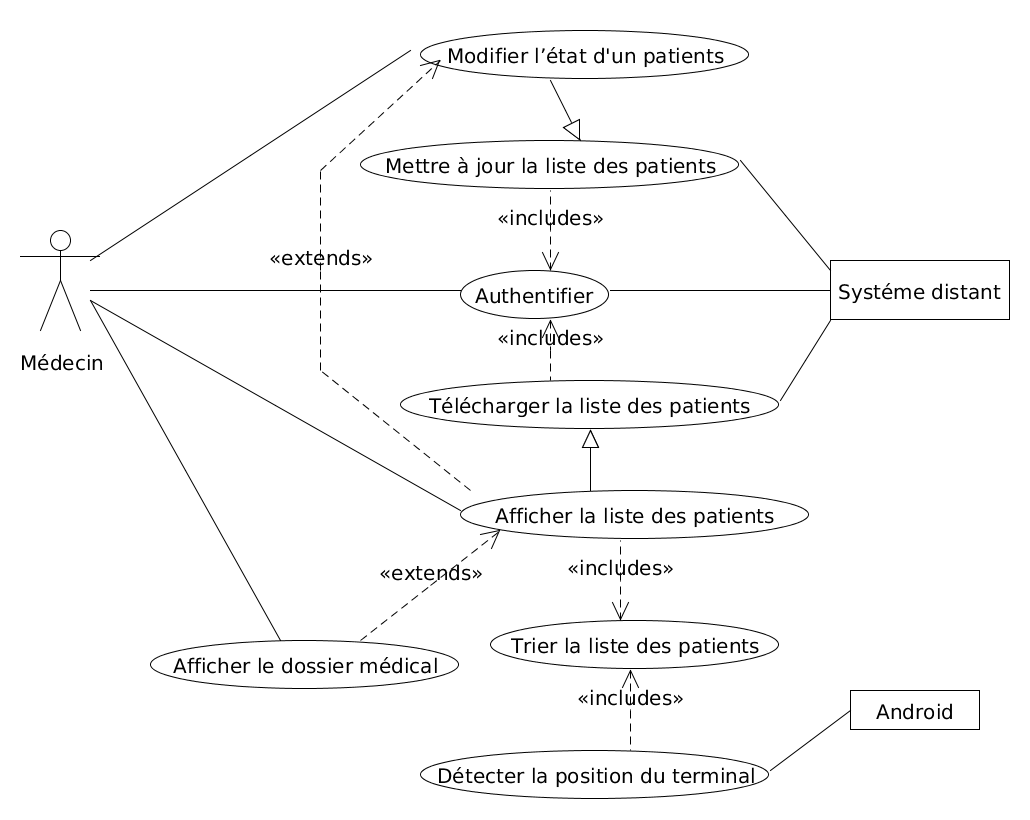
\includegraphics[width=0.8\textwidth]{diagrams/usecases}
\caption{Diagramme \gls{uml} des cas d'utilisation.}
\label{fig:usecase}
\end{figure}

\subsubsection{Cas: Authentifier}
\subsubsection{Cas: Notifier la proximiter d'un patient}
\subsubsection{Cas: Detecter la position du terminal}
\subsubsection{Cas: Afficher la list des patients}
\subsubsection{Cas: Télecharger la list des patients}
\subsubsection{Cas: Modifier la list des patients}
\subsubsection{Cas: Mettre à jour la list des patients}

\subsection{Environnement de développement}%TODO

\section{Architecture Général}

\begin{figure}
\center
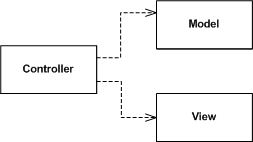
\includegraphics[scale=1]{passive_view}
\caption{Diagramme \gls{uml} du patron \en{Passive Viev}~\cite{fowler:passive_view}}
\label{fig:passive_view}
\end{figure}

L'architecture globale de l'application est calqué sur Le patron "Vue
Passive" (Passive View). Le patron \en{Passive View} (fig
\ref{fig:passive_view}) est une variation des patrons \gls{mvc} et
\gls{mvp}, à ce qui ce passe dans ces patrons l'interface utilisateur
est divisé entre une vu qui s'occupe de l'affichage des données et un
controlleur qui repont aux interactions de l'utilisateur. La différance
majeur avec le \en{Passive View} est que la vue est completemement
passive et n'ai pas responsable de sa mise à jour depuis le model. Dans
ce cas tout la logique de la vue est dans le controlleur et aucune
dependances ni dans un sens au dans un autre entre le vue et le
model~\cite{fowler:passive_view}.

Ce patron est idéal dans notre cas pour deux raisons majeurs:
\begin{itemize} 

\item Dans notre projet le en{view} n'est pas une partie très important
dans la mesure ou l'objectif est d'intégré un système éventuellement
pré-conçu, donc avec une autre logique de présentation. Déporter les
interactions avec le modèle dans le contrôleur permet d'intégrer
d'autre implémentation d'affichage plus facilement.

\item La nature même de cette procédure d'accés - a savoir l’aspect
abstrait, donc plus fragile - nous pousse à réduire les composants en
relations pour réduire la marge d'erreur possible et facilité les tests.

\end{itemize} 

Dans la suite de ce chapitre, on procède à l'explication détaillés de chaque composant de cette architecture.

\section{Le Modèle} 


Un des objectifs de ce projet étant de fournir une solution d’accès au
donnée flexible à fin de couvrir les besoins de chaque client de manière
individuel. On a opter donc pour un modèle basé sur l’implémentation de
deux interfaces (figure \ref{fig:adl}):

\begin{itemize}
\item Interface d'authentification.
\item Interface d’accès à la liste des patients.
\end{itemize}

\begin{figure}
\center
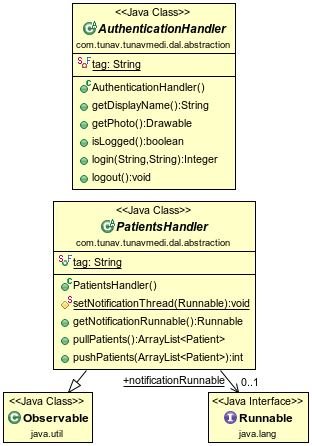
\includegraphics[width=0.8\textwidth]{diagrams/cls_adl}
\caption{Diagramme de classe de la couche d'accées.}
\label{fig:adl}
\end{figure}

L'idée est simple: pour chaque client, une implémentation spécifique à son infrastructure sera développez soit par son propre effectif, soit par une des équipes de Tunav, ou dans le cas idéale par une alliance formé par des agents des deux camps qui garantie une collaboration plus poussée pour des résultats meilleurs.
Ces ensemble d'interfaces nous permet de construire notre application 

\subsection{Implémentation de test} 

\begin{figure}
\center
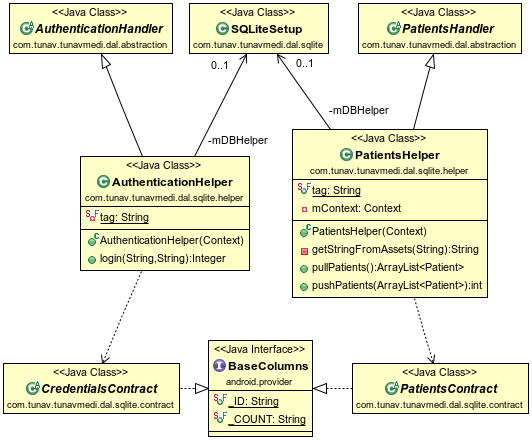
\includegraphics[width=0.8\textwidth]{diagrams/cls_adl_sqlite}
\label{fig:adl_sqlite}
\caption{Diagramme de classe de l'implémentation de la couche d'accées de test à base de SQLite.}
\end{figure}

Une implémentation de la couche d’accès abstraite est réalisé dans le
cadre de ce projet pour pouvoir testé la solution. Cette implémentation
est de caractère locale à l'application à travers les \gls{api} de la
base de données \dev{SQLite} qui fait parti de l'\gls{sdk} \android{}.
En fait une implémentation locale nous affranchies des problèmes qui
peuvent se produire dont la corrélation avec l'application est faible.
Cette même idée a influencé la mise en place même de cette
implémentation qui à su rester la plus simple possible en restant très
proches des objets de base de notre application.

Se trouvant dans le package \dev{com.tunav.tunavmedi.dal.sqlite}, cette implémentation peut être subdivisé en trois éléments:

\begin{description}
\item[Les Contrats] représente les contrats relative aux tables dans notre implémentation de test. chaque contrat implémente l'interface \dev{android.provider.BaseColumns} et contient - entre autre - les commandes SQL de création et de suppression de la dite table, des éventuel index, et les commande d'insertion des données de test.

\item[Les \en{Helpers}] ce sont les implémentations des classes
abstraites qui définisse la couche d’accès et présente les procédure d'extraction des données pré-inséré dans nos table fictives en faisant appel à la classe \dev{SQLiteSetup} .

\item[la classe \dev{SQLiteSetup}] Elle hérite de la classe \dev{SQLiteOpenHelper} et destiner à contrôler la création et l’accès à notre base de données de teste.
\end{description}

\subsection{Interface d'authentification}

\subsection{Interface des Données}
\subsubsection{Mécanisme de notification}

\begin{figure}[H]
\center
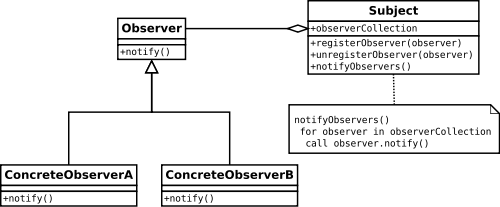
\includegraphics[width=0.8\textwidth]{Observer}
\caption{diagramme UML du patron de conception Observateur~\cite{wiki:observer}}
\label{fig:observer}
\end{figure}

Le patron \textbf{Observateur} (\en{observer pattern}) (fig \ref{fig:observer}) et un patron de conception couramment utilisé et qui nous perment d'avoir une relation 1/N entre divers objets.
Le patron observateur assume que l'objet qui contient les données est séparé des l'objets qui les affiche et ces dites objets \en{observe} le changement de ces données~\cite{jdp-observer}.
Quant on implémente le patron observateur, on réfère communément à l'objet contenant les données par "Sujet"; et chacun des consommateurs des données par "Observateur", Et chaque Observateurs implémente une interface préconnu que le Sujet invoque quant les données changes~\cite{jdp-observer}.
Dans le langage Java, ce patron est réaliser à travers la class \dev{java.util.Observable} et l'interface \dev{Java.util.Observer}. Le Sujet hérite de la classe \dev{Observable} et les changements sont signalé par les méthodes \dev{setChanged()} et \dev{notifyObservers()} ou \dev{notifyObservers(Object message)}.

%TODO show in our code

\section{Le Contrôleur}

\section{La Vue}
Le système d'exploitation \android rend facile le développement des application qui tourne sur des appareils qui possèdes des forme et des taille d’écran différents, une des amélioration

\section{Testes}

\subsection[Pourquoi tester?]{Pourquoi tester? ~\cite{pycon:getting_started_with_automated_testing}}

\begin{itemize}
\item La raison la plus évidente pour écrire les testes - étant la plus populaires aussi - est que c'est un moyen efficace pour savoir si le bout de code ajouté dans le projet marche correctement ou pas, ce qui non seulement fournit une certaine confiance dans la robustesse du logiciel mais présente un effet secondaire bénéfique en réduisant le temps nécessaire pour le débogage à la recherche d'un bug caché. %FIXME
\item Une autre raison pour écrire les testes est que c'est un autre forme de documentation qui aide les autres développeurs comprendre le code contenu dans le projet.
\item Une raison non évidente pour écrire des teste est le fait que les tests améliore la manière dont le code est conçu en mettant en évidence les difficultés pour le maintenir.
\end{itemize}
\subsubsection{Modifié la localisation dans l'émulateur}%FIXME

\subsection{Quelque difficultées rencontrées}

\section{Conclusion du chapitre}
%!TEX root = report.tex

\chapter*{Conclusion Générale}   
\addcontentsline{toc}{chapter}{Conclusion Générale}

L’intégration des technologies au sein des établissements médicaux est, malgré les divers obstacles, une tendance établie et représente un marché juteux pour les sociétés désirant le conquérir, et justifiant la judicieuse idée derrière ce projet.
Il en demeure que l’application en elle-même reste limitée. Et particulièrement, le processus de déploiement suggère un minimum d’infrastructures requises. Donc pour offrir l’expérience désirée, une solution alternative de support développée par TUNAV est de rigueur pour combler le manque dans les équipements de l’établissement  client ou, dans les cas extrêmes les supplanter. Une stratégie de commercialisation est un besoin évidant.
Ce projet peut être qualifié de type \og{}proof of concept\fg{}, il vise à explorer une idée et vérifier son applicabilité. Une aubaine pour l’application produite qui, en toute honnêteté, n’est pas encore au point et souffre de plusieurs lacunes de conceptions et d’implémentation. Si un produit sérieux dans le même thème est à offrir par TUNAV, des efforts de recherche et de développement sont de mise. En particulier l’intégration de médecins pratiquants dans des hôpitaux au processus de conception et de tests serait   critique pour la compétitivité du produit. 
Cependant, les problèmes techniques pour le développement de cette application ne sont pas les seuls à freiner son adoption. Outre le problème de coûts et l’effort de persuasion requis, c’est un problème d’ordre psychologique auquel il faut  faire face. En effet, avec tout concept qui change radicalement des procédures bien établies, une réticence de la part des utilisateurs ciblés, en l’occurrence les médecins, et le staff médical dans un contexte plus large, risque de saboter  les tests d´intégrations. Des campagnes  de sensibilisation sont à prévoir. 

%!TEX root = report.tex
\appendix

\chapter{UI/Application Exerciser Monkey}
\label{chptr:monkey}

\begin{lstlisting}[language=bash, label=lst:adb_monkey, caption=Utilisation de l'UI/Application Exerciser Monkey]

$ adb shell monkey -v -p com.tunav.tunavmedi 300
:Monkey: seed=1371512317847 count=300
:AllowPackage: com.tunav.tunavmedi
:IncludeCategory: android.intent.category.LAUNCHER
:IncludeCategory: android.intent.category.MONKEY
// Event percentages:
//   0: 15.0%
//   1: 10.0%
//   2: 2.0%
//   3: 15.0%
//   4: -0.0%
//   5: 25.0%
//   6: 15.0%
//   7: 2.0%
//   8: 2.0%
//   9: 1.0%
//   10: 13.0%
:Switch: #Intent;action=android.intent.action.MAIN;category=android.intent.category.LAUNCHER;launchFlags=0x10200000;component=com.tunav.tunavmedi/.activity.MainActivity;end
    // Allowing start of Intent { act=android.intent.action.MAIN cat=[android.intent.category.LAUNCHER] cmp=com.tunav.tunavmedi/.activity.MainActivity } in package com.tunav.tunavmedi
:Sending Touch (ACTION_DOWN): 0:(190.0,120.0)
:Sending Touch (ACTION_UP): 0:(191.60419,128.55092)
:Sending Trackball (ACTION_MOVE): 0:(3.0,-3.0)
:Sending Touch (ACTION_DOWN): 0:(473.0,23.0)
:Sending Touch (ACTION_UP): 0:(473.1426,23.805832)
:Sending Trackball (ACTION_MOVE): 0:(-5.0,3.0)
:Sending Trackball (ACTION_MOVE): 0:(3.0,0.0)
:Sending Trackball (ACTION_MOVE): 0:(-3.0,-5.0)
:Sending Touch (ACTION_DOWN): 0:(5.0,341.0)
:Sending Touch (ACTION_UP): 0:(4.349031,340.68045)
:Sending Trackball (ACTION_MOVE): 0:(2.0,-3.0)
:Sending Touch (ACTION_DOWN): 0:(611.0,766.0)
    //[calendar_time:2013-06-05 10:14:32.168  system_uptime:1098585565]
    // Sending event #100
:Sending Touch (ACTION_UP): 0:(678.4827,701.28955)
:Sending Touch (ACTION_DOWN): 0:(680.0,240.0)
:Sending Touch (ACTION_UP): 0:(669.64984,250.41994)
:Sending Trackball (ACTION_MOVE): 0:(1.0,2.0)
:Sending Trackball (ACTION_MOVE): 0:(-3.0,4.0)
:Sending Touch (ACTION_DOWN): 0:(33.0,339.0)
:Sending Touch (ACTION_UP): 0:(20.433603,303.77527)
:Sending Trackball (ACTION_MOVE): 0:(-4.0,-2.0)
:Sending Touch (ACTION_DOWN): 0:(556.0,636.0)
:Sending Touch (ACTION_UP): 0:(592.86835,561.529)
:Sending Trackball (ACTION_MOVE): 0:(2.0,2.0)
:Sending Touch (ACTION_DOWN): 0:(233.0,837.0)
:Sending Touch (ACTION_UP): 0:(226.95929,825.0325)
:Sending Touch (ACTION_DOWN): 0:(71.0,554.0)
:Sending Touch (ACTION_UP): 0:(73.91967,528.69226)
:Sending Touch (ACTION_DOWN): 0:(30.0,341.0)
:Sending Touch (ACTION_UP): 0:(84.22933,308.51373)
    //[calendar_time:2013-06-05 10:14:32.873  system_uptime:1098586237]
    // Sending event #200
    //[calendar_time:2013-06-05 10:14:32.874  system_uptime:1098586238]
    // Sending event #200
:Sending Trackball (ACTION_MOVE): 0:(1.0,-2.0)
:Sending Trackball (ACTION_MOVE): 0:(-3.0,0.0)
:Sending Trackball (ACTION_UP): 0:(0.0,0.0)
:Sending Touch (ACTION_DOWN): 0:(782.0,261.0)
:Sending Touch (ACTION_UP): 0:(789.2555,259.95465)
:Sending Touch (ACTION_DOWN): 0:(480.0,1180.0)
:Sending Touch (ACTION_UP): 0:(517.4512,1113.8969)
:Sending Touch (ACTION_DOWN): 0:(775.0,965.0)
:Sending Touch (ACTION_UP): 0:(762.51733,968.3565)
:Sending Trackball (ACTION_MOVE): 0:(4.0,-4.0)
:Sending Trackball (ACTION_MOVE): 0:(1.0,-2.0)
:Sending Trackball (ACTION_MOVE): 0:(-3.0,1.0)
:Sending Touch (ACTION_DOWN): 0:(89.0,1185.0)
:Sending Touch (ACTION_UP): 0:(109.65848,1195.4576)
:Sending Trackball (ACTION_MOVE): 0:(-4.0,-5.0)
:Sending Touch (ACTION_DOWN): 0:(339.0,280.0)
:Sending Touch (ACTION_UP): 0:(351.69287,274.5476)
:Sending Trackball (ACTION_MOVE): 0:(0.0,-1.0)
Events injected: 300
:Sending rotation degree=0, persist=false
:Dropped: keys=0 pointers=0 trackballs=0 flips=0 rotations=0
## Network stats: elapsed time=1986ms (0ms mobile, 1986ms wifi, 0ms not connected)

\end{lstlisting}

\chapter{Logiciel de gestion de versions Git}

\begin{figure}
\center

\includegraphics[width=0.4\textwidth]{git_logo}
\caption{Logo du logiciel de gestion de version Git}
\label{fig:git}
\end{figure}

\en{Git}\cite{wikipedia:git} est un système de gestion de versions et un gestionnaire de code source connu pour sa rapidité. Conçu et développée initialement par \textsf{Linus Torvalds} pour le développement du \en{Kernel} \en{Linux}, Git a depuis éte adopter par plusieurs autre projets.

Chaque répertoire de travail de Git est un dépôt complet avec un historique complet et des capacité de suivit de version, il est indépendant d'un accès réseau ou d'un serveur centrale.

Git est un logiciel libre distribuer sous les termes de la licence  \en{GNU General Public License} version 2.

L'usage de Git est très simple, un des workflow simplifier serai comme suit:

\begin{itemize}

\item La branche master contient la dernière version de l'application. Malheureusement, cette version contient un bug dans le \dev{MenuItem}

\item Pour éviter, pendant qu'on corrige le bug, d'altérer la version courante de  l'application de façon nuisible, on crée une branche différente ou on peut tester nos modification tranquillement (listing \ref{lst:git_branch}).

\item On peut passer vers la nouvelle branche crée précédemment (listing \ref{lst:git_checkout}).

\item On à maintenant réussi a corrigé le bug en question, et aussi travailler un peut sur notre rapport. On peut avoir un rapport sur les fichiers modifier pendant ce processus (listing \ref{lst:git_status}).

\item Après on peut appliquer nos changements dans la branche master de notre répertoire Git (listing \ref{lst:git_merge}).

\end{itemize}

\begin{lstlisting}[language=bash, label=lst:git_branch, caption=Git Branch]

\end{lstlisting}

\begin{lstlisting}[language=bash, label=lst:git_checkout, caption=Git checkout]

\end{lstlisting}

\begin{lstlisting}[language=bash, label=lst:git_status, caption=Git status]

➜  PFE git:(bug_MenuItem) ✗ git status

# On branch bug_MenuItem
# Changes not staged for commit:
#   (use "git add <file>..." to update what will be committed)
#   (use "git checkout -- <file>..." to discard changes in working directory)
#
#   modified:   README.md
#   modified:   pfe.sublime-project
#   modified:   report/2_cadre_general.tex
#   modified:   report/4_travail.tex
#   modified:   report/acronyms.tex
#   modified:   report/appendix.tex
#   modified:   report/bibliography.bib
#   modified:   report/report.pdf
#   modified:   report/report.tex
#   modified:   res/ep/Scenarios.ep
#   modified:   res/ep/architecture.ep
#   modified:   source/tunavmedi/src/com/tunav/tunavmedi/fragment/PatientListFragment.java
#
# Untracked files:
#   (use "git add <file>..." to include in what will be committed)
#
#   res/architecture-interfaces.png
#   res/ep/scenarioactors.png
#   res/ep/scenarioalltunav.png
#   res/ep/scenariointeractions.png
#   res/ep/scenarioother.png
#   res/sc_display.png
#   res/sc_options.png
#   res/sc_urgent.png
no changes added to commit (use "git add" and/or "git commit -a")

\end{lstlisting}

\begin{lstlisting}[language=bash, label=lst:git_merge, caption=Git merge]

\end{lstlisting}

\bibliography{bibliography}
\label{LastPage}

\end{document}
